\documentclass{beamer}

\mode<presentation>
{
  \usetheme{Warsaw}
  \setbeamercovered{transparent}
}


\usepackage{subcaption}
\usepackage{hyperref}
\usepackage[english]{babel}
\usepackage[utf8]{inputenc}
\usepackage{times}
\usepackage[T1]{fontenc}
\usepackage{graphicx}
\usepackage{tikz}
\usepackage{float}

\usetikzlibrary{fit}
\graphicspath{ {./images/} }

\title[An Implementation of Hypersuccinct Trees]
{An Implementation of Hypersuccinct Trees}

\author{Christopher Pack, Alexander Auras, Nathanael Stöhr, Charbono Lonyem Tegomo}
\institute[Universität Siegen]
{
  Lehrstuhl für theoretische Informatik\\
  Universität Siegen}
\date{\today}

\everymath{\displaystyle}

\AtBeginSection[]
{
  \begin{frame}
    \frametitle{Table of Contents}
    \tableofcontents[currentsection]
  \end{frame}
}

\begin{document}

\begin{frame}
  \titlepage
\end{frame}

\begin{frame}{Outline}
  \tableofcontents
\end{frame}

\section[Introduction]{Introduction}

\begin{frame}{Introduction}
	\begin{itemize}
	\item
	We were tasked with creating an implementation of a hypersuccinct tree encoding, as described in \cite{farzanMunro}.
	\item
	Additionally we add the possibility of huffman encoding for part of the tree, to provide an implementation of the encoding improvement mentioned in \cite{universalSuccinct}.
	\item
	Our result is a library that can encode trees in acceptable time, and is able to perform queries on those encoded trees in $O(1)$, while offering huffman encoding for their Microtrees.
	\end{itemize}
\end{frame}

\section{Theory}

\subsection[Hypersuccinct Tree Code]{Hypersuccinct Tree Code}

\begin{frame}{The tree covering Algorithm} %Muss genauer sein!!!!
\begin{itemize}
	\item
		Given a splitting size $m$, all resulting trees are at most of size $2m$.
	\item
		The resulting subtrees at most share a single node, their root.
	\item
		Most subtrees' roots lie either directly below other subtree roots or share roots with other subtrees, and a dictionary of the root's children can be used to identify tree connections.
	\item
		Subtrees that do not lie directly at or below other roots require a special node, a Dummy, to represent their connection to its higher tree.
	\end{itemize}
\end{frame}

\begin{frame}{The tree covering Algorithm}
\begin{figure}[t]
	\includegraphics[scale=0.2]{TreeCovering}
\caption{Example of Tree decomposition with $m = 5$ \cite{farzanMunro}}
\end{figure}
\end{frame}

\begin{frame}{The tree covering Algorithm}
	To fully decompose a tree for hypersuccinct encoding, \cite{farzanMunro} offers the following procedure:
	\begin{itemize}
	\item
		First decompose the entire tree into Minitrees with the size $\lceil lg^{2} n \rceil$.
	\item
		Generate the FIDs and Dummys for their interconnections.
	\item
		Then decompose each Minitree into Microtrees with the size $\lceil \frac{lg n}{8} \rceil$.
	\item
		Generate the FIDs and Dummys for their interconnections.
	\end{itemize}
\end{frame}
%introduce Lookuptable

\begin{frame}{Queries}
	As mentioned in \cite{farzanMunro}, additional data needs to be saved in order to execute queries without needing to decode hypersuccinct trees.
	\begin{itemize}
	\item
		Additional query data is saved for each level of abstraction (Minitrees, Microtrees, individual nodes).
	\item
		To execute some queries, navigation on the FID and the Typevector is required.
		\begin{itemize}
			\item
				As the definition of "Fully Indexable Dictionary" states, it is necessary to implement \textit{Rank} and \textit{Select} queries.
			\item
				A possible efficient implementation is described in \cite{succinctBV}, which is implemented in an external library \cite{succinctBVLink}.
		\end{itemize}
	\end{itemize}
\end{frame}

\section{Our Implementation}

\subsection{Our hypersuccinct tree}

\begin{frame}{Hypersuccinct nodes and trees}
%Bild of Struktur oder so
	\begin{itemize}
	\item
		Hypersuccinct nodes are tripels that represent their Minitree, Microtree, and Node within the Microtree.
	\item
		The Hypersuccinct\_Tree class implements the encoding and offers the query functions.
	\item
		The Hypersuccinct Factory handles creating a hypersuccinct tree from possible sources.
	\end{itemize}
\end{frame}

\begin{frame}{The Hypersuccinct Factory}
	\begin{itemize}
	\item
		The hypersuccinct factory encodes trees efficiently, making use of multiple threads with a multithreading library \cite{threading}.
	\item
		Creates data for query execution.
	\item
		The hypersuccinct factory also creates hypersuccinct trees from an encoded file. Since an already encoded file is read, there is no processing for generating any data.
	\end{itemize}
\end{frame}

\begin{frame}{FIDs and specific issues}
	\begin{figure}[h]
	\begin{tabular}{ |p{2.4cm}||p{0.6cm}|p{0.6cm}|p{0.6cm}|p{0.6cm}|p{0.6cm}|p{0.6cm}|p{0.6cm}|p{0.6cm}|  }
		 \hline
		 Bitvector & Bit 1 &Bit 2&Bit 3&Bit 4& Bit 5 &Bit 6&Bit 7&Bit 8\\
		 \hline
		 Minitree FID 0 & 1 & 1& 0 & 1 & 0 & 0 & 1 & 1\\
		 Minitree TV 0& 0 & 1 & - & 0 & - & - & 1 & 0\\
		 Minitree Nr. & 0 & 3 &  0 & 1 & 1 & 1 & 5 & 2\\
		 \hline
		 Minitree FID 1 & 1 & 0& 1 & 1 & 0 & 1 & 1 & 1\\
		 Minitree TV 1& 0 & - & 1 & 1 & - & 1 & 1 & 0\\
		 Minitree Nr. & 3 & 3 &  6 & 7 & 3 & 8 & 9 & 4\\
		 \hline
	\end{tabular}
	\caption{Indices for Minitrees}
	\end{figure}
\end{frame}
%Just explain on image?
\begin{frame}{FIDs and specific issues}
	\begin{itemize}
		\item
		To solve the discrepancies with FID and tree indices:
		\begin{itemize}
			\item
				Bitvectors that denote the first Type 0 (Top) and Type 1 (Low) tree of every FID.
			\item
				Bitvectors the denote their Top and Low FIDs for each Tree.
			\item
				This is done for both Mini- and Microtrees, so 8 bitvectors in total.
		\end{itemize}
		\item
			To solve the issue with identifying the correct low trees:
		\begin{itemize}
			\item
				When identifying trees, we always take the top tree of the FID that the low index points to. 
			\item
				This is possible since each FID points to its first low tree, which points to its own FID, and other low FIDs have incremental indices by construction.
		\end{itemize}
	\end{itemize}
\end{frame}

\begin{frame}{Minitrees and Lookuptable entries}
	\begin{itemize}
	\item
		Minitrees and Lookuptable entries are structs that hold bitvectors.
	\item
		Minitrees hold all information for their Microtrees, all their query data and all their Microtree query data.
	\item
		Lookuptable entries hold information of their structure and a key for identification, as well as query data.
	\end{itemize}
\end{frame}



\subsection{Queries}

\begin{frame}{Simple Queries}
	Simple queries are such that require only one bitvector per abstraction. Their structure simply moves from one abstraction level to the next one to answer the query.\\
	These simple queries are:
	\begin{itemize}
	\item[1)] \textit{getParent}
	\item[2)] \textit{degree}
	\item[3)] \textit{subtreeSize}
	\item[4)] \textit{depth}
	\item[5)] \textit{height}
	\item[6)] \textit{leftmostLeaf}
	\item[7)] \textit{rightmostLeaf}
	\item[8)] \textit{leafSize}
	\item[9)] \textit{levelSuccessor (Not implemented)}
	\item[10)] \textit{levelPredecessor (Not implemented)}
	\end{itemize}
\end{frame}

\begin{frame}{Rank Queries}
	Rank queries are queries that return some sort of rank from the tree. These queries are all similar in structure, and need multiple bitvectors per level of abstraction, due to special cases.\\
	These rank queries are:
	\begin{itemize}
	\item[1)] \textit{childRank}
	\item[2)] \textit{leafRank}
	\item[3)] \textit{nodeRank (Not implemented)}
	\end{itemize}
\end{frame}

\begin{frame}{Special cases: Rank}
	\begin{figure}[ht]
	\begin{subfigure}{2cm}
		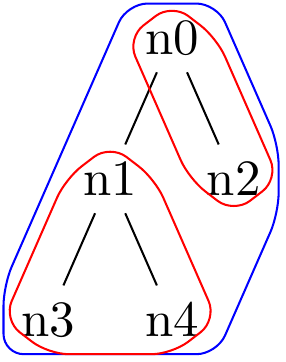
\includegraphics[scale=0.22]{F4C1Tree}
		\caption{Case 1}
		\label{rank:subim1}
	\end{subfigure}
	\begin{subfigure}{2cm}
		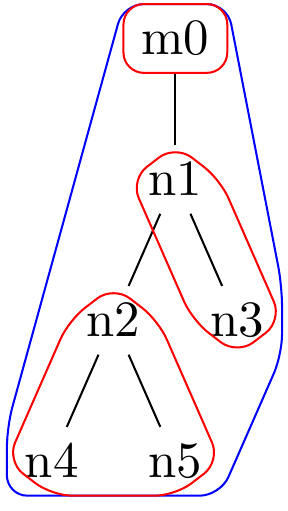
\includegraphics[scale=0.21]{F4C2Tree}
		\caption{Case 2}
		\label{rank:subim2}
	\end{subfigure}
	\begin{subfigure}{3cm}
		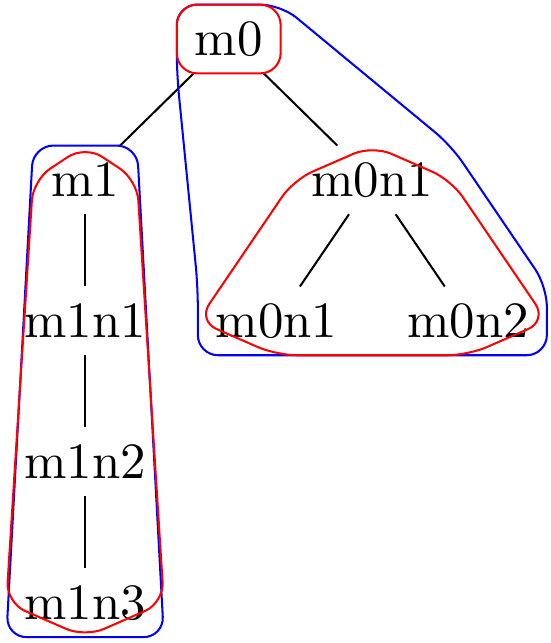
\includegraphics[scale=0.2]{F4C3Tree}
		\caption{Case 3}
		\label{rank:subim3}
	\end{subfigure}
	\begin{subfigure}{3cm}
		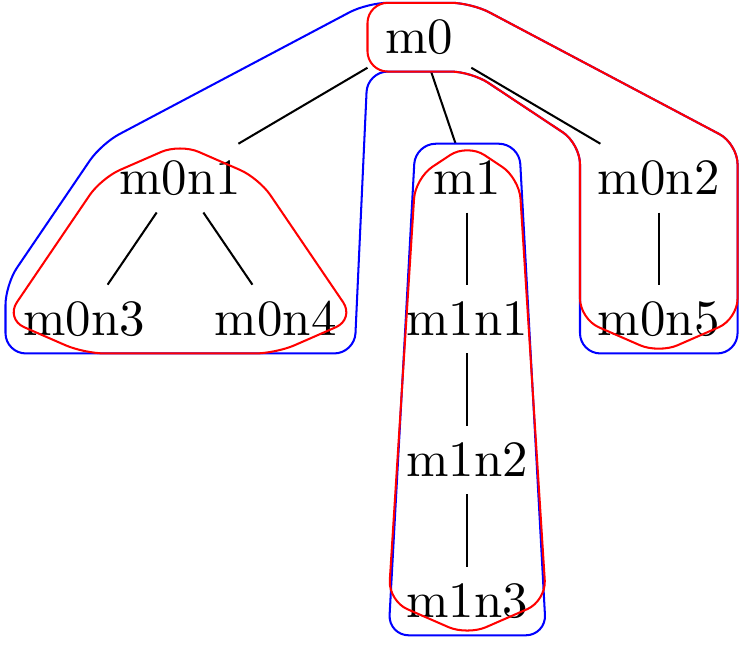
\includegraphics[scale=0.2]{F4C4Tree}
		\caption{Case 4}
		\label{rank:subim4}
	\end{subfigure}

	\caption{4 Special Cases for Rank Queries}
	\label{rank:images4}
	\end{figure}
\end{frame}

\begin{frame}{Special Cases: Rank}
	\begin{itemize}
	\item
		We can use the FID to identify each special case. However, since rank queries do not provide an index in for the FID, the identification of the right position of the node in the FID is difficult, and we therefore need to provide an answer from the node indices alone.
	\item
		We need specific bitvectors that denote the rank of the first child of a tree for data to resolve these cases.
	\item
		We do not need two bitvectors in the lookup table. If \textit{Case 4} only has one Microtree in the higher Minitree, the respective lookuptable will already present the correct result for \textit{m0n2}.
	\end{itemize}
\end{frame}

\begin{frame}{Child}
	This is a very unique query, as it is simpler than rank queries, since the index provided points to direct positions on the FIDs:
	\begin{itemize}
	\item
		We can identify the correct node by moving through the Minitree FID, then the Microtree FID and then the lookuptable entry.
	\item
		Dummy nodes can easily be skipped both at the end and the beginning of the query.
	\end{itemize}
\end{frame}

\begin{frame}{Helper Queries}
	These queries are purely used within other queries to take on some repeat tasks:
	\begin{itemize}
	\item[1)] \textit{isDummyAncestorWithinMiniTree}
	\item[2)] \textit{isDummyAncestorWithinMicroTree}
	\item[3)] \textit{getParentForQuery}
	\end{itemize}
\end{frame}

\section{Tests}

\begin{frame}{Query tests}
	\begin{figure}[H]
	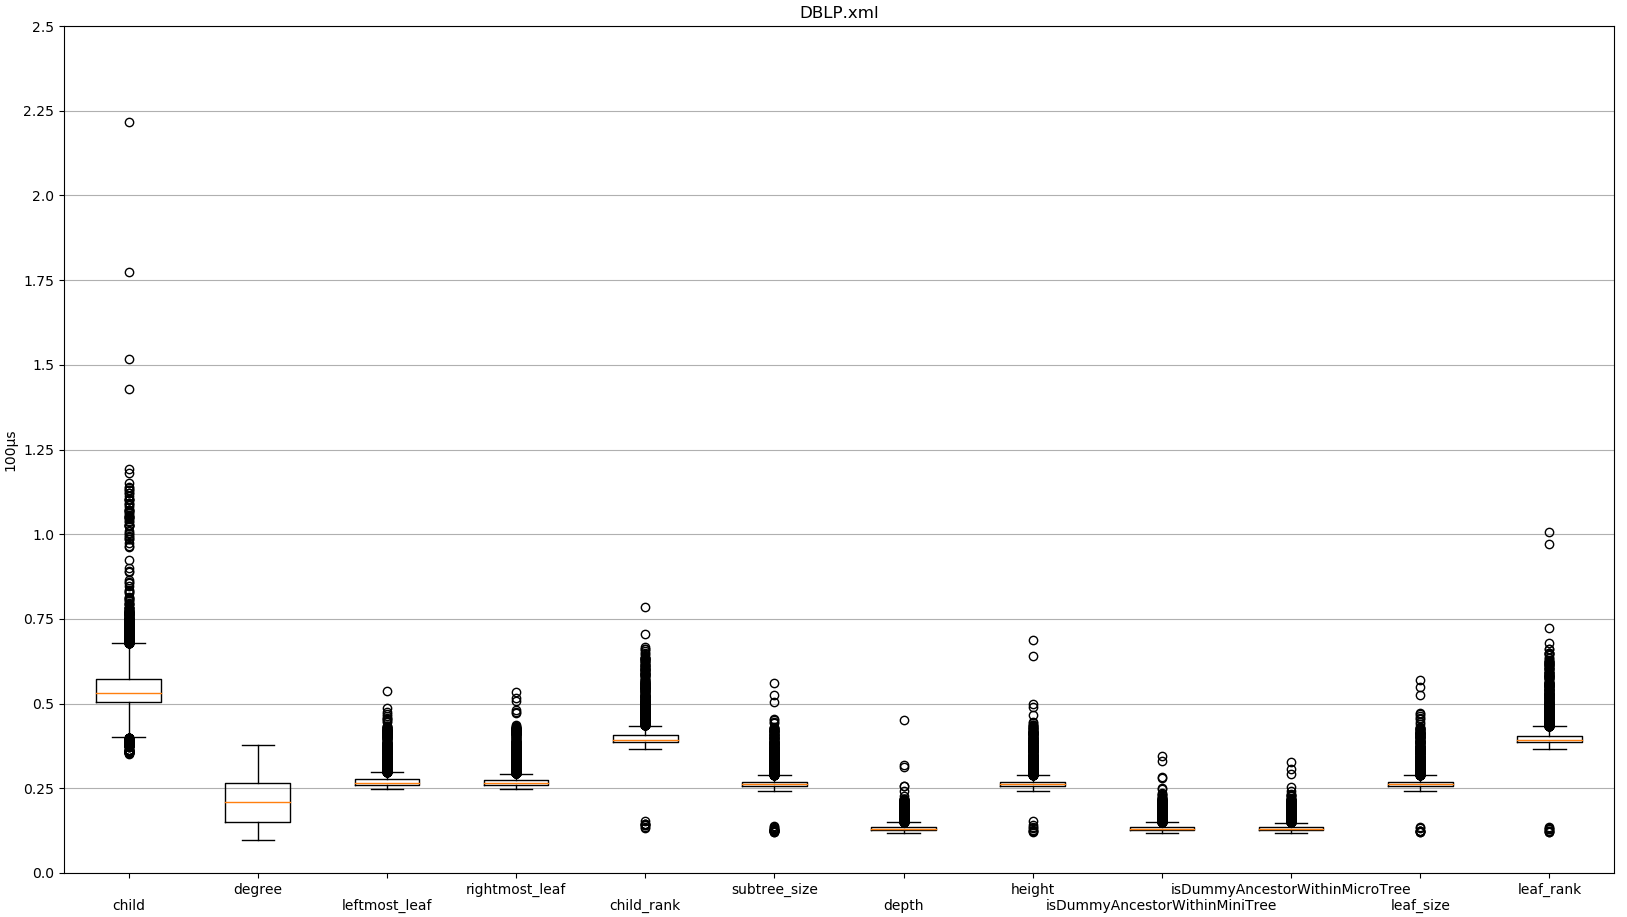
\includegraphics[scale=0.25]{DBLP_Queries}
	\caption{Runtime of implemented queries}
	\label{complexQue:image1}
	\end{figure}
\end{frame}

\begin{frame}{Query tests}
	\begin{itemize}
	\item
		All queries except \textit{child} maintain an anverage runtime below $100 \mu s$.
	\item
		The runtime of \textit{child} actually increases with larger trees. We identified the reason for this being a simple \textit{getMinitree} function, which is also used in multiple other queries.
	\end{itemize}
\end{frame}

\begin{frame}{create, writing and reading}
	\begin{itemize}
	\item
		The encoding process in \textit{create} has been optimized as much as we think possible.
		\begin{itemize}
		\item
			While the \textit{farzan-munro algorithm} cannot be optimized with multithreading, the creation of Microtrees are individual tasks that can be parallelized.
		\item
			Adding huffman encoding decreases efficiency slightly.
		\end{itemize}
	\item
		Reading and writing files is straightforward and therefore much more efficient.
		\begin{itemize}
		\item
			 Writing just pushes every vector with Elias-Gamma encoding into a file.
		\item
			Reading just decodes the vectors from the file. There is no handling of badly formatted vectors.
		\end{itemize}
	\end{itemize}
\end{frame}

\begin{frame}{create, writing and reading}
	\begin{figure}[H]
	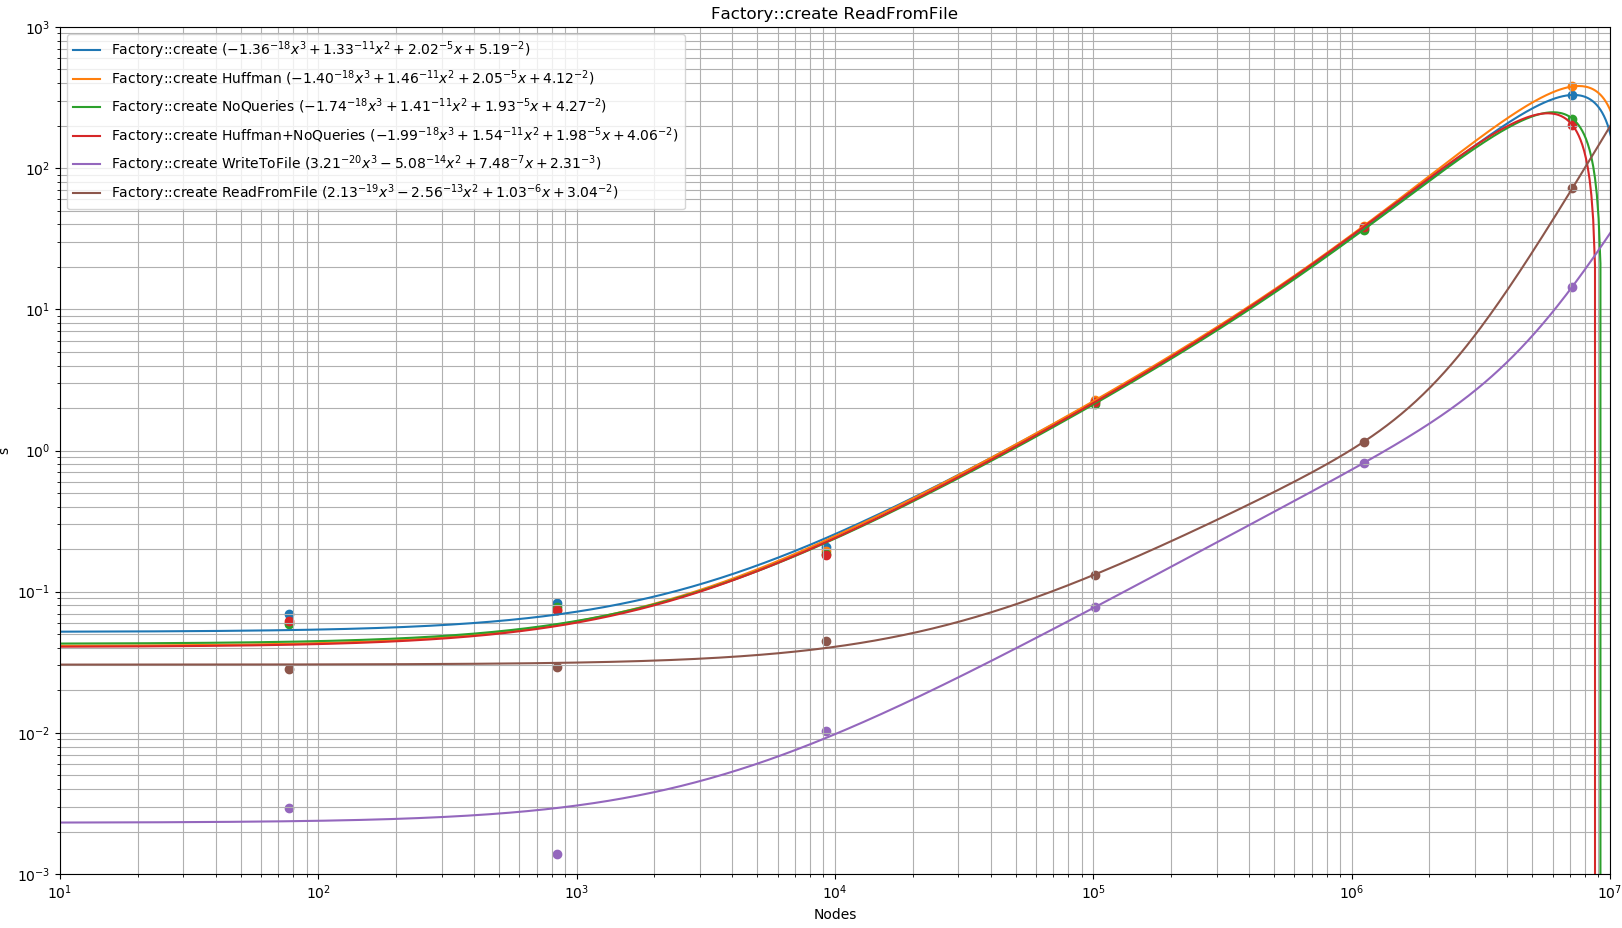
\includegraphics[scale=0.25]{file_compare_cut}
	\caption{Runtime of create, reading and writing}
	\label{complexQue:image1}
	\end{figure}
\end{frame}

\begin{frame}{Space and Huffman}
	\begin{figure}[h]
	\begin{tabular}{ |p{2cm}||p{1.7cm}|p{1.7cm}|p{4cm}|  }
		 \hline
		 Tree Name & Normal &Huffman &Huffman + Lookuptable\\
		 \hline
		 TreeNath   & 52    & 23 &   24 \\
		 TreeNath3&5196 &2695&  2706\\
		 TreeNath4&53369& 31709&  31732\\
		 TreeNath5&583289&345005&345029\\
		 XMark2&2004196&831572&831627\\
		 DBLP&3690039&593804&593842\\
		 \hline
	\end{tabular}
	\caption{Space for normal encoding and huffman encoding in byte}
	\label{huff:table1}
	\end{figure}
	\begin{itemize}
	\item
		Space reduction is fairly obvious.
	\item
		XMark2 is larger than DBLP with huffman due to having more evenly distributed tree structures.
	\end{itemize}
\end{frame}

\section{Demonstration}
\begin{frame}
	-- Demonstration of program --
\end{frame}
%USE PYTHON INTERFACE HERE

\section*{Conclusion}
%Do we need conclusion if demonstration comes before it? We could end on demo
\begin{frame}{Conclusion}
	\begin{itemize}
	\item
		We have created a library that can encode trees succinctly.
	\item
		Our tree encoding is space efficient and allows us to execute various queries in $O(1)$.
	\item
		We offer huffman encoding for our tree, which saves space.
	\item
		The encoding process is optimized, can encode trees with more than 7 million nodes in less than 6 minutes.
	%Sketch - 6 minute figure applies to 16 parallel threads
	\end{itemize}
\end{frame}

\begin{frame}[allowframebreaks]{References}
	\bibliographystyle{IEEEtran}
	\bibliography{references}
\end{frame}

\end{document}


